\documentclass[
	letterpaper
	12pt
]{template}

\usepackage{apacite}
\usepackage{titling}
\usepackage{wrapfig}
\usepackage[font=footnotesize,labelfont=bf]{caption}

\setlength{\droptitle}{-10em}
\newcommand{\bref}[2]{\textbf{\hyperref[#1]{#2}}}

\begin{document}

\title{Motion in Fluids}

\author{Sebastien Psarianos, Yuchen Jiang}

\date{\today}
\maketitle
\section{Abstract}
In this experiment, we aimed to quantitatively examine the accuracy the terminal velocity predictions made by low and high Reynolds number approximations. This was done through the analysis of the terminal velocity of beads falling through a high Reynolds number environment (water) and a low Reynolds number environment (glycerine). Over the course of the analysis, fits of the data to the corresponding model in both experiments resulted in low $\chi_{red}^2$ values, suggesting that there was validity in the proportional predictions of the model. However, there were large inaccuracies in the proportionality constant in both situations. This was likely due to issues that were encountered within the experiment at high terminal velocities, due to the limitation of the video tracking apparatus that was used. To further verify the validity of this model, a more high quality video tracking apparatus should be employed.

\section{Introduction}
This study explores the field of fluid dynamics by investigating how differing inertial and viscous force ratios, quantified in this experiment by Reynolds Number (\bref{eqn::reynolds}{Equation 1}), affect the drag force experienced by a falling object. Through terminal velocity analysis of spheres with differing sizes falling through both a high and low Reynolds number regime, we hope to provide a quantitative analysis of the accuracy of high and low Reynolds number approximations for drag force (\bref{eqn::dragForce}{Equation 2}).

\subsection{Background}
Reynolds number (\bref{eqn::reynolds}{Equation 1}) is the measure used in this report to quantify whether a system's mechanics are dominated inertial or viscous forces. It is a dimensionless quantity that represents the ratio of inertial to viscous forces, defined as follows:
\begin{equation}\label{eqn::reynolds}
	R_e = \frac{\rho l v}{\eta}\ \ \text{\cite{batchelor_2002}}
\end{equation}
Where $\rho$ represents density $l$ is the objects size $v$ is its speed and $\eta$ is the fluid density. An object falling at terminal velocity can be modelled as the velocity where the drag force $F_d(v)$ and the gravitational force $mg$ are equal:
\[mg = F_d(v_{t})\]
Applying this terminal velocity condition to both an idealized high and low Reynolds number system, one can derive the following approximations for drag force in both regimes:
\begin{align}\label{eqn::dragForce}
	F_d(v) = 6\pi\eta r v \text{ (Low $R_e$)} && F_d(v) = {1\over 2}\rho C_dAv^2 \text{ (High $R_e$)} && \cite{labManual}
\end{align}
Where $C_d$ is an empirically measured drag coefficient, $\rho$ is fluid density, $A$ is cross-sectional area and $r$ is the object's radius. Rewriting the mass in terms of volume and density ($m =  {4\over 3}\rho_{\rm s}\pi r^3$), substituting $A=\pi r^2$ then solving for $v_{\rm term}$ gives the following predictions for terminal velocity:
\begin{align}\label{eqn::terminalVelocity}
	v_{\rm term}  = {2\rho_{\rm s} g\over 9 \eta}\cdot r^2 \text{ (Low $R_e$)} && 	v_{term} =\sqrt{8\rho_{\rm s} g\over \rho C_d  3}\cdot \sqrt{r} \text{ (High $R_e$)}
	&& \cite{labManual}
\end{align}

\subsection{The experiment}
In this experiment we used glycerine to simulate a low Reynolds Number regime and water to simulate a high Reynolds Number regime. This choice was made due to water's low density $\eta_{w} \approx 1\times10^{-2}\unit{g\per {\cm\second}}$ in comparison to glycerine $\nu_g \approx 9.34\unit{g\per {\cm\second}}$ \cite{labManual}. Since \bref{eqn::reynolds}{Reynold's Number} is inversely related to fluid viscosity, water will have a comparatively larger Reynolds Number than  glycerine for a given velocity/size scale. By measuring terminal velocity of spheres of varying radii falling through both fluids, we aim to quantitatively examine the accuracy the terminal velocity predictions in \bref{eqn::terminalVelocity}{Equation 3}, derived from the drag force predictions in \bref{eqn::dragForce}{Equation 2}.


\section{Methodology}
\subsection{Apparatus}

\begin{wraptable}{r}{0.5\textwidth}
	\vspace{-23pt}
	\begin{flushright}\label{tab::beadSize}
		\begin{tabular*}{.5\textwidth}{@{\extracolsep{\fill}}  |c|c|c|}
			\hline
			\textbf{Bead} & \textbf{Radius (Water)} & \textbf{Radius (Glycerine)}\\
			\hline
			1&$(2.35\pm0.01)\unit{mm}$&$(1.55\pm0.01)\unit{mm}$\\
			2&$(3.13\pm0.01)\unit{mm}$&$(2.39\pm0.01)\unit{mm}$\\
			3&$(3.92\pm0.01)\unit{mm}$&$(3.13\pm0.01)\unit{mm}$\\
			4&$(4.72\pm0.01)\unit{mm}$&$(4.70\pm0.01)\unit{mm}$\\
			5&$(6.27\pm0.01)\unit{mm}$&$(6.30\pm0.01)\unit{mm}$\\
			\hline
		\end{tabular*}
		\caption{Reference bead sizes}
	\end{flushright}
	\vspace{-20pt}
\end{wraptable}


For each fluid, the terminal velocity of differing size categories of beads numbered $1\rightarrow 5$ were tested. Teflon beads were used for the glycerine tank and Nylon beads were used for the water tank. These materials were chosen for their densities and minimal water absorption properties, allowing them to maintain consistent shape and weight during the experiment. Every bead that were measured in each size category had a similar radius to the order of $\pm 0.05\unit{mm}$.  \bref{tab::beadSize}{Table 1} contains one sample radius from each size category for the Nylon and Teflon beads used in the respective experiment.\vspace{\baselineskip}

\begin{wrapfigure}{r}{0.35\textwidth}\label{fig::apparatus}
	\centering
	\vspace{-10pt}
	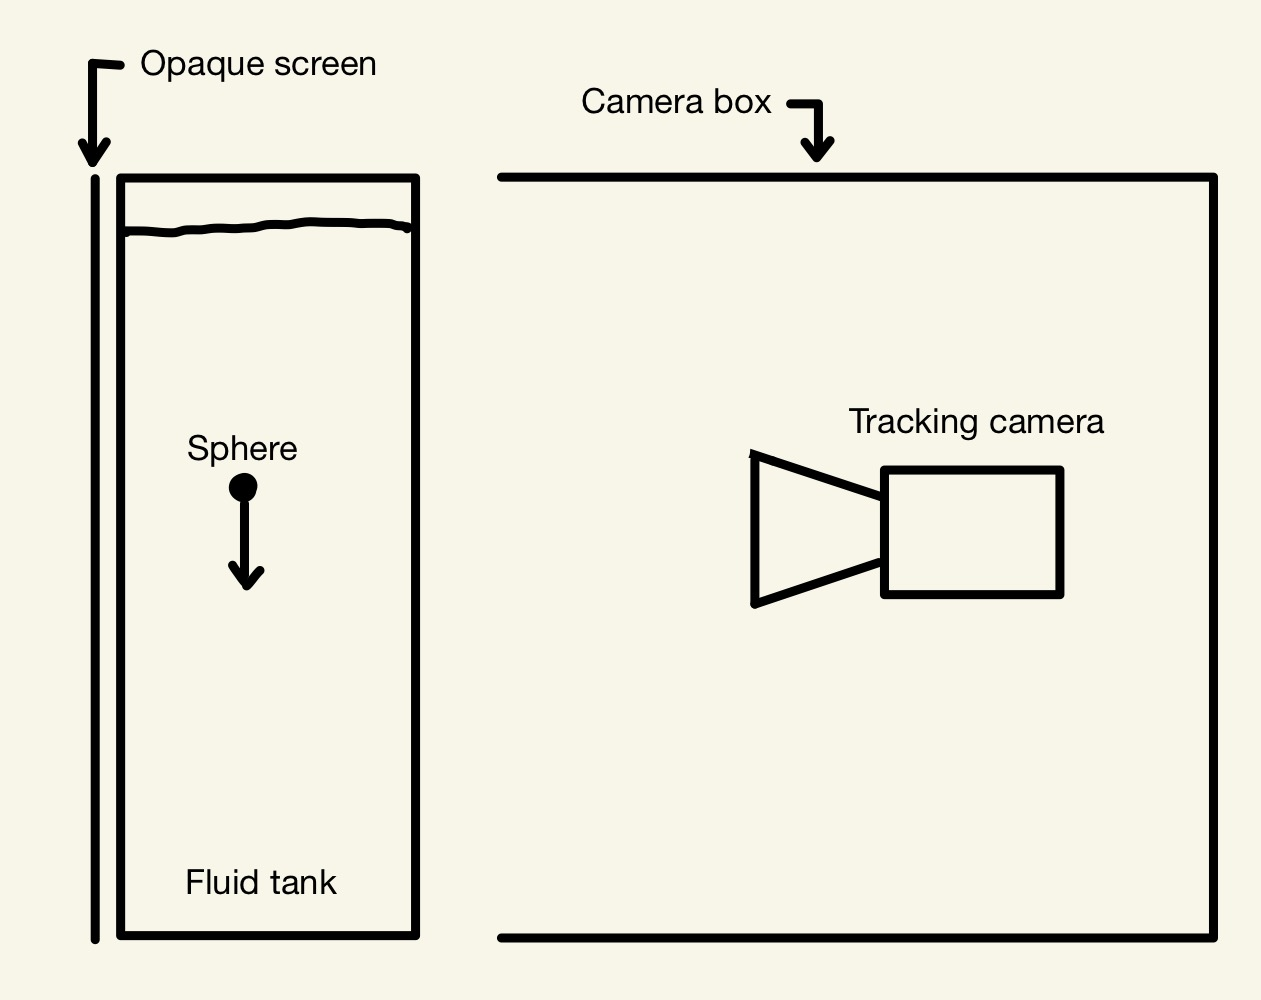
\includegraphics[width=.35\textwidth]{figures/apparatus.jpg}
	\caption{Diagram of apparatus}
	\vspace{-20pt}
\end{wrapfigure}
The vessel that was used to contain the fluid that was being tested was a transparent, rectangular tank. On one side of this container, an opaque screen was attached that completely covered that side of the container. The use of this screen in conjunction with the white color of the beads created a high contrast environment for optimal video tracking. \vspace{\baselineskip}

A camera was set up in an opaque box, opposing the opaque screen. There was an opening in the box that allowed the camera to view the interior of the tank. The camera's frame rate was changed in each trial to strike a balance between high time resolution and managing file sizes. A diagram of this apparatus is displayed in \bref{fig::apparatus}{Figure 1}. The video recording and tracking were performed using a purpose built LabView applet called "Motion through Fluids" provided with the apparatus.
\subsection{Procedure}
\subsubsection{Initial time estimates}\label{sec::timeEst}
Prior to starting the experiment, we dropped one bead from each of the five size categories into its corresponding fluid and timed how long it took to reach the bottom of the tank. This gave a rough estimate of how long each trial would take, informing the choice of video duration and frame rate for each sample.
\subsubsection{Trial Process}
For both fluids, we performed three trials for each of the 5 bead sizes, giving 15 total glycerine samples and 15 total water samples. The following procedure was followed for all of these trials: \vspace{\baselineskip}

First, the diameter of the bead was measured using a set of calipers. Since it was non-trivial to measure the widest part of the bead and determine the diameter, three measurements were taken for each bead and the largest value measured was the one that was used. Using the total decent time detailed in \bref{sec::timeEst}{2.2.1} determined for the specific bead-size/fluid combination, an appropriate frame count and frame-rate was chosen within the software. After the video tracking had been started in the software, the bead was carefully released in the center of the container using a set of tweezers. Once the video tracking process had ended, the LabView applet returned a text document containing the position vs time.
\vspace{\baselineskip}

Through the course pre-experimental trial runs, two adjustments were made to the process. Releasing the bead on top of the fluid gave a noticeable increase in test duration, likely due to surface tension. Therefore, care was taken to release the bead under the surface of the fluid to minimize these effects. Additionally, tracking tended to have issues tracking the bead right after it started. Therefore, the bead was released a short duration after the video had started, and this pre-drop data was removed after the fact.
\section{Results and Analysis}
\subsection{Calculating Terminal Velocity}

The data that was given by the LabView applet contained position values corresponding to specific timestamps. Therefore, to calculate the terminal velocity, some further processing was required. For every position measurement, the average velocity between that measurement and the measurement four points after was calculated using $v_{avg} = \Delta x/ \Delta t$. The average velocity was taken over a four measurement gap to reduce the amount of velocity uncertainty as detailed in \bref{sec::uncertainty}{Section 3.2}. This process resulted in $n-1$ approximate velocity measurements for $n$ position measurements. \vspace{\baselineskip}

\begin{wrapfigure}{r}{0.5\textwidth}\label{fig::terminalPlotG}
	\vspace{-30pt}
	\centering
	\includegraphics[width=0.55\textwidth]{../python/output/terminalPlotG.pdf}
	\caption{Terminal velocity of a teflon bead falling through a glycerine tank (mm/s) vs bead radius (mm). Terminal velocity was measured by taking the average velocity over every four measurement intervals. These velocities were sorted, and the largest velocity was plotted for each sample. A fit is included of \bref{eqn::terminalVelocity}{Equation 3} (The low reynold number radius velocity relation approximation).}
	\vspace{-50pt}
\end{wrapfigure}
After some filtering of the data set was done to compensate for tracking issues (detailed in \bref{sec::filtering}{Section 3.3}), this set of velocity measurements, the largest value was chosen to be the terminal velocity and plotted using matplotlib. Using curve\_fit from the scipy.optimize module a regression was performed on both sets of terminal velocities. For the glycerine data set, this was done using \bref{fnc::squaredFit}{squaredFit}, a python implementation of the low Reynolds Number terminal velocity approximation (\bref{eqn::terminalVelocity}{Equation 3}).

\begin{lstlisting}[label={fnc::squaredFit},captionpos=b,language=python]
def squaredFit(x, A):
	return A * x **2
\end{lstlisting}

For the water data set, this was done using \bref{fnc::sqrtFit}{sqrtFit}, a python implementation of the high Reynolds Number terminal velocity approximation (\bref{eqn::terminalVelocity}{Equation 3}).\vspace{0pt}

\begin{lstlisting}[label={fnc::sqrtFit}, captionpos=b,language=python]
	def sqrtFit(x, A):
		return A * np.sqrt(np.abs(x))
\end{lstlisting}

The resulting plots for the glycerine and water data sets are shown in \bref{fig::terminalPlotG}{Figure 2} and \bref{fig::terminalPlotW}{Figure 3} respectfully. Both plots display the best fit coefficient and the $\chi_{red}^2$ metric as a goodness of fit measure. The uncertainties of the fit variables in both plots were calculated by taking the square root of the corresponding value in the covariance matrix supplied by the curve\_fit function. Additionally, \bref{fig::terminalPlotGRes}{Figure 4} and \bref{fig::terminalPlotWRes}{Figure 5} are the resulting residual plots.

\subsection{Uncertainty}\label{sec::uncertainty}

\begin{wrapfigure}{r}{0.5\textwidth}\label{fig::terminalPlotW}
	\vspace{-32pt}
	\centering
	\includegraphics[width=0.55\textwidth]{../python/output/waterMaxGraph.pdf}
	\caption{Terminal velocity of a nylon bead falling through a water tank (mm/s) vs bead radius (mm). Terminal velocity was measured by taking the average velocity over every four measurement intervals. These velocities were sorted, and the largest velocity was plotted for each sample. A fit is included of \bref{eqn::terminalVelocity}{Equation 3} (The high Reynolds number radius velocity relation approximation).}
	\vspace{-20pt}
\end{wrapfigure}

After an analysis of the variance in the position measurements, a position uncertainty of $\pm 0.05$ for any position measurements that were made. To account for the discrete nature of position tracking using a camera, the time uncertainty was set to $\pm 0.25 \cdot \Delta t_f$, where $\Delta t_f$ is the time between frames.\vspace{\baselineskip}

Considering all terminal velocity values were calculated using the expression $v_{avg} = {\Delta x\over \Delta t}$ with $\Delta x = x_1 - x_0$ and $\Delta t = t_1 - t_0$. The uncertainty of $\Delta x$ and $\Delta t$ can be first calculated from \bref{eqn::sumUnc}{Equation 4} \cite{harrison_2023}:
\begin{equation}\label{eqn::sumUnc}
	u(x+y) = \sqrt{[u(x)]^2 + [u(y)]^2}
\end{equation}
Applying this equation to the previously calculated values for
\begin{align*}
	u(\Delta x) &= \sqrt{u(x_1)^2 + u(x_0)^2} = 0.07\\
	u(\Delta t) &= \sqrt{u(t_1)^2 + u(t_0)^2} = {t_f/ \sqrt 8}
\end{align*}
The uncertainty of $\Delta x/\Delta t$ can be calculated using relative error propagation (\bref{eqn::relError}{Equation 5}) \cite{harrison_2023}.
\begin{equation}\label{eqn::relError}
	{u(x/y)\over x/y} = \sqrt{\left({u(x)\over x}\right)^2+\left({u(y)\over y}\right)^2}
\end{equation}
Plugging in uncertainty values, this gives:
\[u(v) = v\sqrt{\left({0.07\over \Delta x}\right)^2+\left({t_f/\sqrt{8}\over \Delta t}\right)^2}\]
Which was used to propagate all velocity values. For example, the first size 4 sample that was taken had values: $v = 11.2mm/s$, $t_f = 0.05s$, $\Delta t = 0.2s$, $\Delta x = 2.25mm$. Therefore, the error value was given:
\[u(v) = (11.22) \cdot \sqrt{\left({0.07\over 2.25}\right)^2+\left({0.05/\sqrt{8}\over 0.2}\right)^2} \approx 1\]
This procedure was repeated for every velocity value that was calculated. The size measurements' uncertainty was set to $\pm0.01\unit{mm}$ as this was the least significant figure on the caliper readings.\vspace{\baselineskip}

During the first pass of analysis, the velocity uncertainties were found to be quite large. After some investigation, this was found to be due to the fact that the uncertainty of $\Delta t$ was very high in comparison to the value of $\Delta t$, resulting in a high velocity uncertainty when these values are put in \bref{eqn::relError}{Equation 5}. Therefore, the velocity calculations were taken over a longer interval of $4$ position measurements to increase $\Delta t$ relative to its uncertainty.
\subsection{Data Filtering}\label{sec::filtering}
As the particle speed increased in the water trials, the software would occasionally lose track the bead's position. When this occurred, it would default to $0mm$ and then return to the bead's position when it was next detected, resulting in inaccurate velocities. In an effort to reduce the effect on the final data set, the decision was made to try to filter out these data points. This was done in two main ways.\vspace{\baselineskip}

The first filtering method was to remove any position measurements with a position of $0$. All starting position values of the data sets were nonzero and $0$ was only measured when the tracker lost track of the bead and therefore there was no effect on physical data measurements. Since all position measurements were timestamped, removing measurements did not affect any velocity calculations other than making the time interval they were averaged over slightly larger.\vspace{\baselineskip}

After plotting velocity vs time graphs for each sample, we noticed that every sample had a clear asymptotic trend to a terminal velocity. This was interrupted however by extremely large velocity values that were clearly due to tracking issues and not physical measurements. We decided to remove any velocity measurement with an absolute value greater than 2.5 times the mean velocity. This resulted in a clear asymptotic terminal velocity in all data sets. This filtering was only applied to the water data set as all large tracking issues occurred in these samples.
\section{Discussion}
\subsection{Glycerine Experiment}
In \bref{fig::terminalPlotG}{Figure 2}, the model seems to fit the data quite well. This is confirmed with the value of $\chi_{red}^2=0.9952$. This suggests that the quadratic proportionality between radius and velocity suggested by \bref{eqn::terminalVelocity}{Equation 3} is a good approximation for this system.\vspace{\baselineskip}

For the low Reynolds number approximation used in the glycerine experiment (\bref{fig::terminalPlotG}{Equation 3}), the coefficient that was fit for in the \bref{fnc::squaredFit}{squaredFit} function should be equal to $2\rho_s g \over 9\eta$. Plugging in known values for the variables, $\rho_s = 2.2\unit{g\per cm^3}$, $g = 9.8\unit{m\per s} $, $\eta = 9.34\unit{g \per{ cm \cdot s}}$ \cite{labManual}
\begin{align*}
	{2\rho_s g \over 9\eta} &= {2(2.2\unit{g \per cm^3})(9.8\unit{m\per s^2}) \over 9(9.34 \unit{g\cdot cm^{-1}\cdot  s^{-1} })} \approx 5.1\unit{mm^{-1}\cdot s^{-1}}
\end{align*}

\begin{wrapfigure}{r}{0.4\textwidth}\label{fig::terminalPlotGRes}
	\vspace{-30pt}
	\centering
	\includegraphics[width=.4\textwidth]{../python/output/terminalPlotGRes.pdf}
	\caption{Residual plot for \bref{fig::terminalPlotG}{Figure 2}}
	\vspace{-20pt}
\end{wrapfigure}

The fit value that was measured of $0.502\pm0.008$ was off the model's predictions by an order of magnitude. It is possible that there is a factor that is affecting the results that is not accounted for in the model. It is also possible that this discrepancy occurred due to a calculation error. The calculated value is off by a factor of 10 almost exactly and an incorrect unit conversion somewhere in the process could likely be the cause of this. \vspace{\baselineskip}

\bref{fig::terminalPlotGRes}{Figure 4} shows the residual plot for the experiment. From a visual inspection, there seems to be a slight bias above zero that is created by measurements of the largest bead size that are noticeably further from the fit than previous measurements. As previously discussed, occasionally loss of tracking was encountered, creating false position measurements and becoming more prevalent with higher velocities. These were minimal in the glycerine experiment but were noticed in the trials with the largest bead size. This is likely the cause for this divergence from the model in the last measurement. \vspace{\baselineskip}

The $\chi_{red}^2$ value suggests that the velocities quadratic and square root dependence on radius is a good model, just with the wrong coefficient. Due to this, the calculations that provided the terminal velocity values in \bref{eqn::terminalVelocity}{Equation 3}, the calculations that provided the coefficient value of $5.1\unit{mm^{-1}\cdot s^{-1}}$ and the literature values should all be verified for correctness.

\subsection{Water Experiment}
Analysing \bref{fig::terminalPlotW}{Figure 3}, the fit visually seems to be relatively good, reflected by the $\chi_{red}^2$ value of $1.148$. This suggests that the proportional square root relation between velocity and radius is a good model for this experiment.\vspace{\baselineskip}

For the high Reynolds Number approximation used in the water experiment (\bref{eqn::terminalVelocity}{Equation 3}), the coefficient $A$ from the \bref{fnc::sqrtFit}{sqrtFit} function should have a value of $\sqrt{8\rho_{\rm s} g/ 3\rho C_d  }$. Plugging in the literature values for these variables: $\rho_{\rm s} = 1.12\unit{g \cdot cm^{-3}}$, $\rho = 1\unit{g \cdot cm^{-3}}$, $C_d = 0.5$ \cite{labManual} gives $A\approx  140\unit{\sqrt{mm}\per s}$

\begin{wrapfigure}{r}{0.4\textwidth}\label{fig::terminalPlotWRes}
	\vspace{-10pt}
	\centering
	\includegraphics[width=.4\textwidth]{../python/output/terminalPlotWRes.pdf}
	\caption{Residual plot for \bref{fig::terminalPlotW}{Figure 3}}
	\vspace{-20pt}
\end{wrapfigure}

The computed value from the fit was $58.3\pm 0.9$. This is quite far off of the literature value of $140$. The tracking issues that were present in the experiment were very prevalent in the water data. It is possible that even after the filtering that was done on the data, this still had a large effect on the accuracy of the data. \vspace{\baselineskip}

The residuals plot for the water experiment is displayed in \bref{fig::terminalPlotWRes}{Figure 5}. Although there seems to be a relatively even distribution of measurements above and below the zero value, after visually inspecting the graph it seems as if there is an increasing trend in the residuals. It is possible that a better fit could be achieved through a higher order term of a higher power such as a linear term in addition to the square root term.\vspace{\baselineskip}

\subsection{Reynolds Number}
By applying literature values for the fluid density, fluid viscosity and the measured length/velocity data, the following plots were made of the reynolds number in each trial.
\begin{figure}[H]
	\begin{minipage}[t]{0.4\textwidth}
		\includegraphics[width=\textwidth]{../python/output/reynoldsPlotG.pdf}
		\caption{Plot of calculated reynolds numbers from \bref{eqn::reynolds}{Equation 1} for the glycerine data set}
	\end{minipage}
	\hfill
	\begin{minipage}[t]{0.4\textwidth}
		\includegraphics[width=\textwidth]{../python/output/reynoldsPlotW.pdf}
		\caption{Plot of calculated reynolds numbers from \bref{eqn::reynolds}{Equation 1} for the water data set}
	\end{minipage}\vspace{\baselineskip}

	This confirms that water is an appropriate high Reynolds number approximation and glycerine is an appropriate low Reynolds number approximation.
\end{figure}

\section{Conclusion}
Overall, the data seemed to reflect a clear quadratic dependence in the glycerine trials and a clear square root dependence in the water data with $\chi_red^2$ values of 0.9522 and 1.148 respectively. This suggests that the model is relatively accurate in terms of proportionality. However, to confirm the accuracy of the direct predictions of the model, further testing would be required to verify that the proportionality constant is correct. In a future experiment, steps should be taken to optimize the tracking capabilities of the software at higher speeds, such as using a higher frame rate as this was the main source of inaccuracy for the data tested. Additionally, applying a linear higher order term to the water data could possibly improve the quality of the fit as previously discussed.

\newpage


\newpage
\bibliographystyle{apacite}
\bibliography{references.bib}
\end{document}
